\documentclass[a4paper,12pt]{article}
\usepackage[notoc,noabs]{HaotianReport}

\title{第一次作业:QQ群组数据统计分析}
\author{刘昊天}
\authorinfo{电博181班, 2018310648}
\runninghead{大数据分析(B)课程报告}
\studytime{2018年10月}

\begin{document}
    \maketitle
    %\newpage
    \section{任务1} % (fold)
    \paragraph{问题描述} % (fold)
    Recall and write down the assumptions which one-way ANOVA are based on.
    
    \begin{enumerate}
        \item 独立性:数据是随机采样的,也就是说样本应是相互独立的随机样本;
        \item 正态性:样本残差是正态分布的;
        \item 等方差:各样本采样的总体方差相等。
    \end{enumerate}
    \section{任务2} % (fold)
    \paragraph{问题描述} Focus on two columns: Category (Col[2]) and Average Age (Col[7]). Taking feature Average Age as an example, we want to measure whether the average age varied significantly across the categories. Clearly state the null (H0) and the alternative (H1) hypotheses for this task.
    
    首先对数据进行观察,如\cref{fig:task2-boxplot}所示。可见,对于不同的群主题(类型),平均年龄分布有显著差别。当然,平均年龄分布的平均值差异并不能反映各群主题的平均年龄差异,该图仅能表明平均年龄分布有一定差异。由此,我们对该问题有一定的心理预期(希望用假设检验方法佐证平均年龄分布的差异),这对我们制定H0与H1是有关键影响的。
    \begin{figure}[htbp]
        \centering
        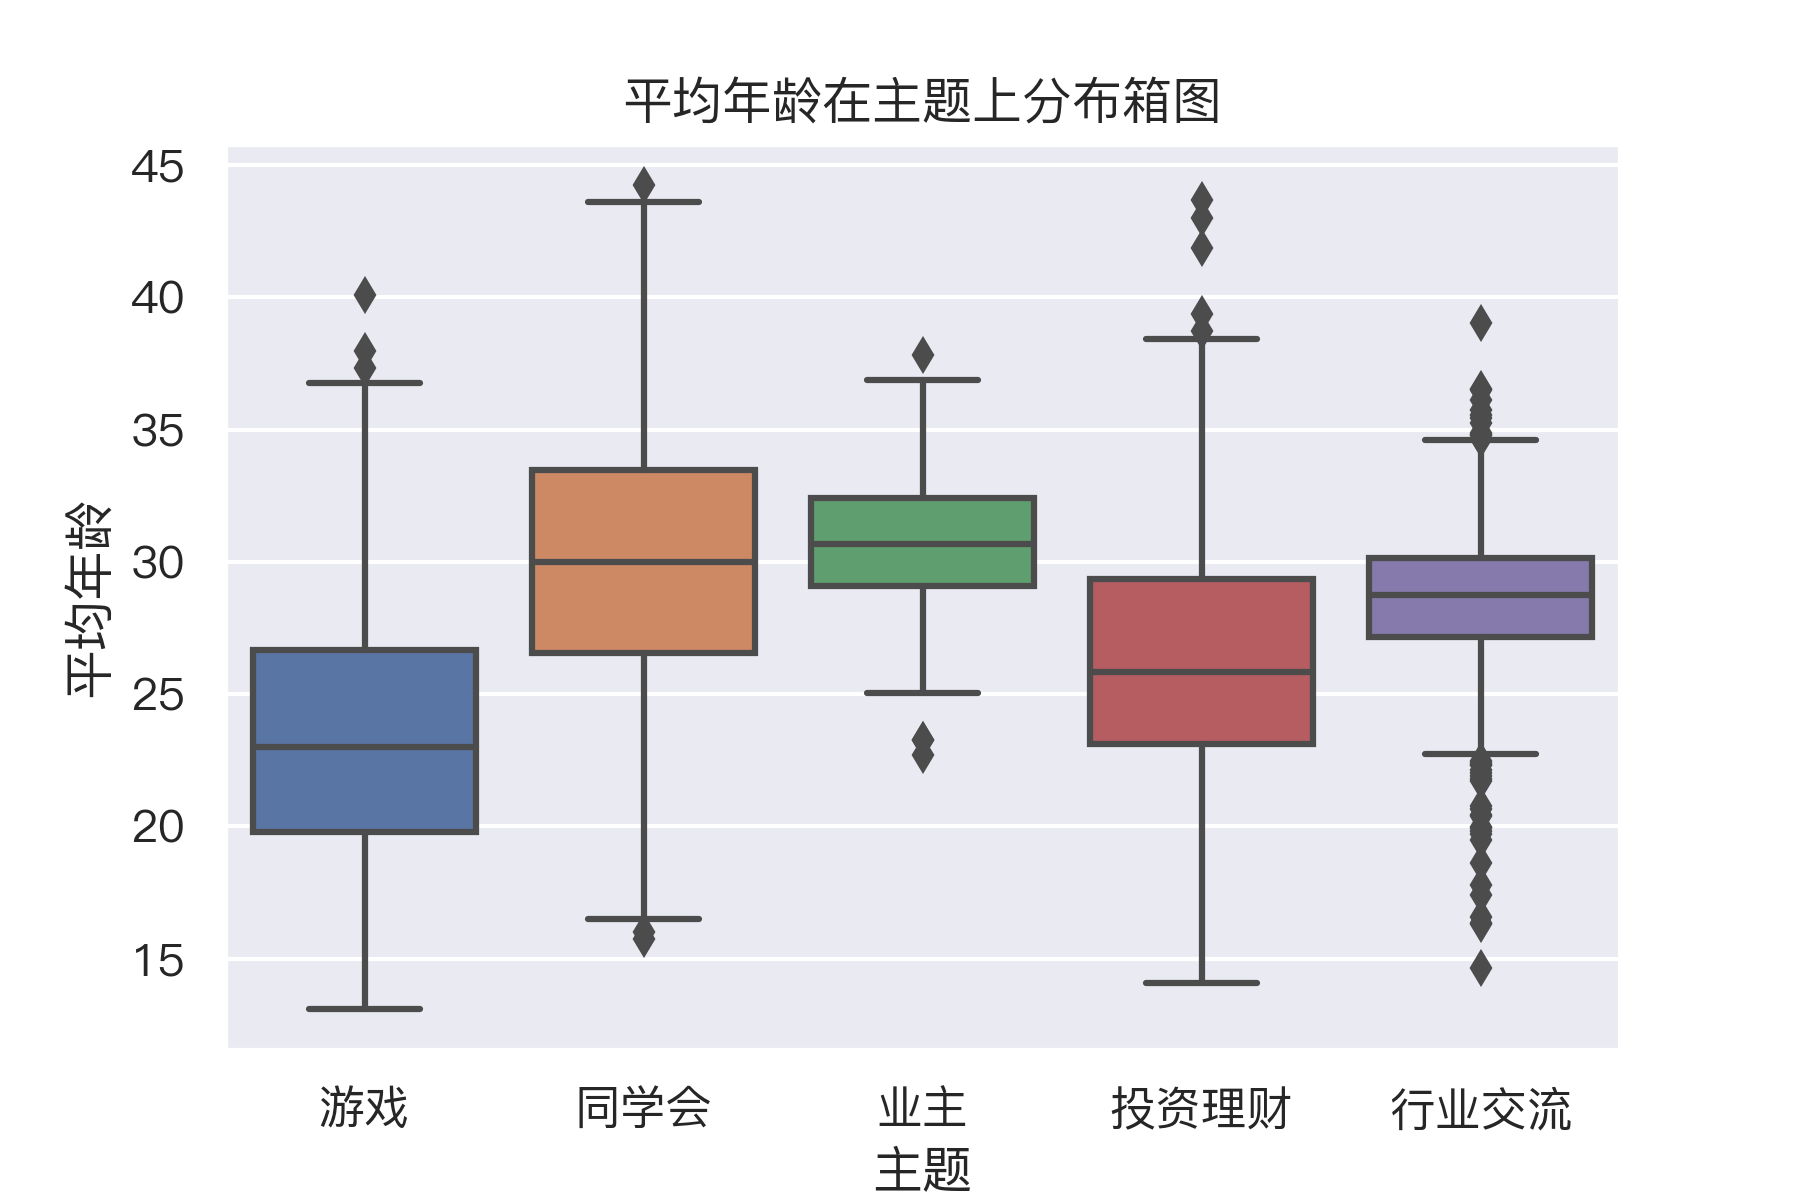
\includegraphics[width=0.95\textwidth]{task2-boxplot}
        \caption{平均年龄随主题变化统计观测}
        \label{fig:task2-boxplot}
    \end{figure}

    由此,我们将两个假设阐述如下:
    \begin{quote}
        H0:不同主题的群之间,平均年龄的分布无显著差异。

        H1:不同主题的群之间,平均年龄的分布差异显著。
    \end{quote}
    
    \section{任务3} % (fold)
    Use your favorite statistics analysis software, like Matlab, R, Excel, SPSS or ...
    \subsection{问题1} % (fold)
    \paragraph{问题描述} Draw the empirical probability density function of Col[7], i.e. the empirical pdf of average age. Does the data in this dimension follow Gaussian distribution? Test normality of Col[7].

    为平均年龄数据绘制直方图及经验概率密度函数,如\cref{fig:task3-pdf}所示。
    \begin{figure}[htbp]
        \centering
        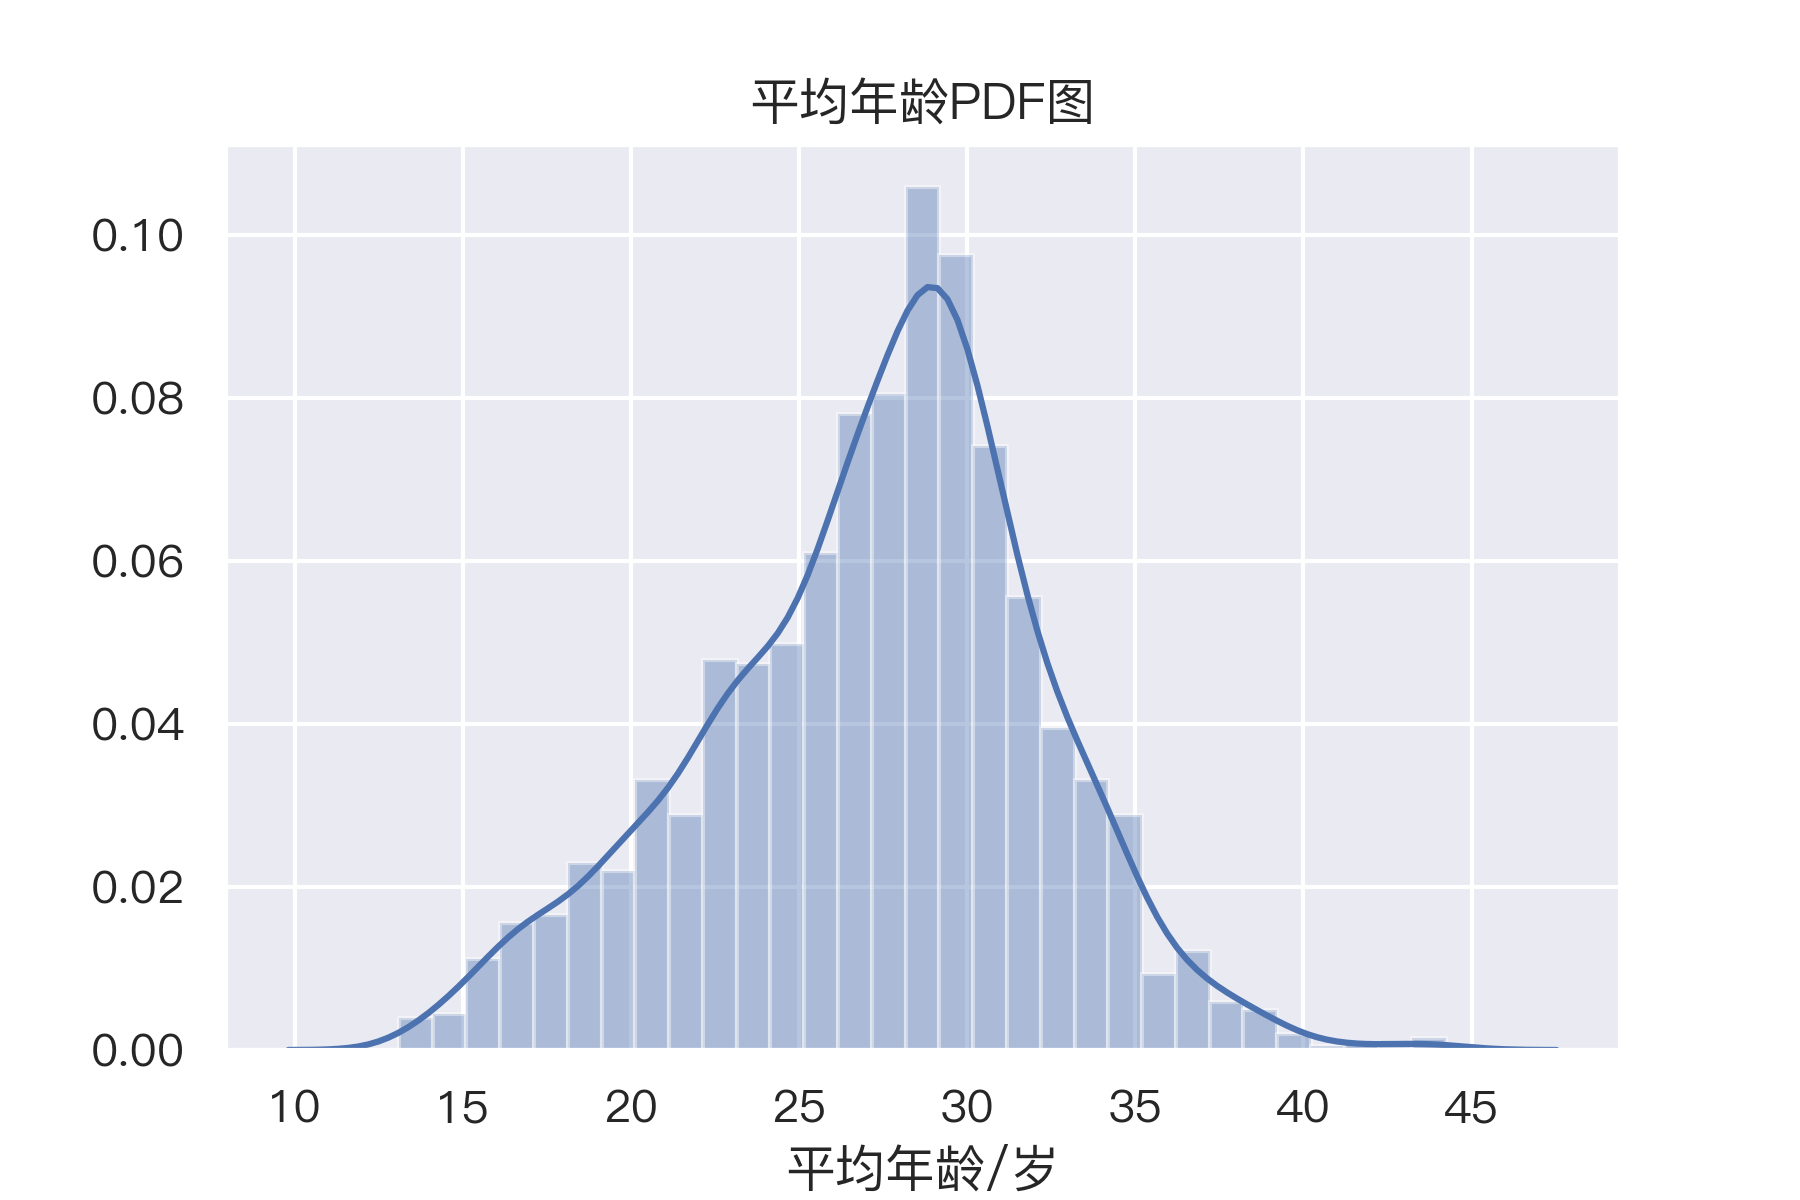
\includegraphics[width=0.95\textwidth]{task3-pdf}
        \caption{平均年龄经验概率密度函数}
        \label{fig:task3-pdf}
    \end{figure}

    可以看到,其相较于正态分布,曲线腰部更瘦,且有明显偏移。为了对该分布的正态性进行验证,可以利用课堂上提到的Skew and Kurtosis Test方法,即偏度-峰度检验。该检验的原假设为“被试分布具有正态性”,备择假设为“被试分布不具备正态性”。得到计算结果如\cref{task4q1log}所示。
    \lstinputlisting[label=task4q1log]{task4q1.log}

    可见,在选取$\alpha=0.05$作为标准时,$pValue<\alpha=0.05$,即有充分把握拒绝原假设,因此该分布不满足正态性。

    \subsection{问题2} % (fold)
    \paragraph{问题描述} In Col[7], there are 5 components divided by category labels. We denote the data in Col[7] with category i (where i = 1,...,5) as Col[7| categoty=i]. Test the normality of each components and test the homogeneity of variances.

    分组后进行同样的检验操作,得到结果如\cref{task4q2log}。可以直接看出,类别编号1,4,5组的平均年龄不满足正态性,类别编号2、3的组可以认为满足正态性。
    \lstinputlisting[label=task4q2log]{task4q2.log}

    对于方差齐的检验,应使用TODO
    \subsection{问题3}
    \paragraph{问题描述} Do the one-way ANOVA test for Col[7] with categories in Col[2]. Write down your conclusion, supporting statistics, and visualize your data which inspire the process.

    利用F检验计算ANOVA,得到结果如\cref{task4q3log}所示。
    \lstinputlisting[label=task4q3log]{task4q3.log}
    TODO

    \section{任务4} % (fold)
    \paragraph{问题描述} Choose another 3 columns, draw the empirical pdf of each feature columns and test which column follows these assumptions in question 1? How about their corresponding log transformation?

    选取性别比、无回应比例以及夜聊比例三组特征,分别给出经验概率密度函数图像,如\cref{fig:gender,fig:noresponse,fig:nightchat}所示。

    \begin{figure}[htbp]
        \centering
        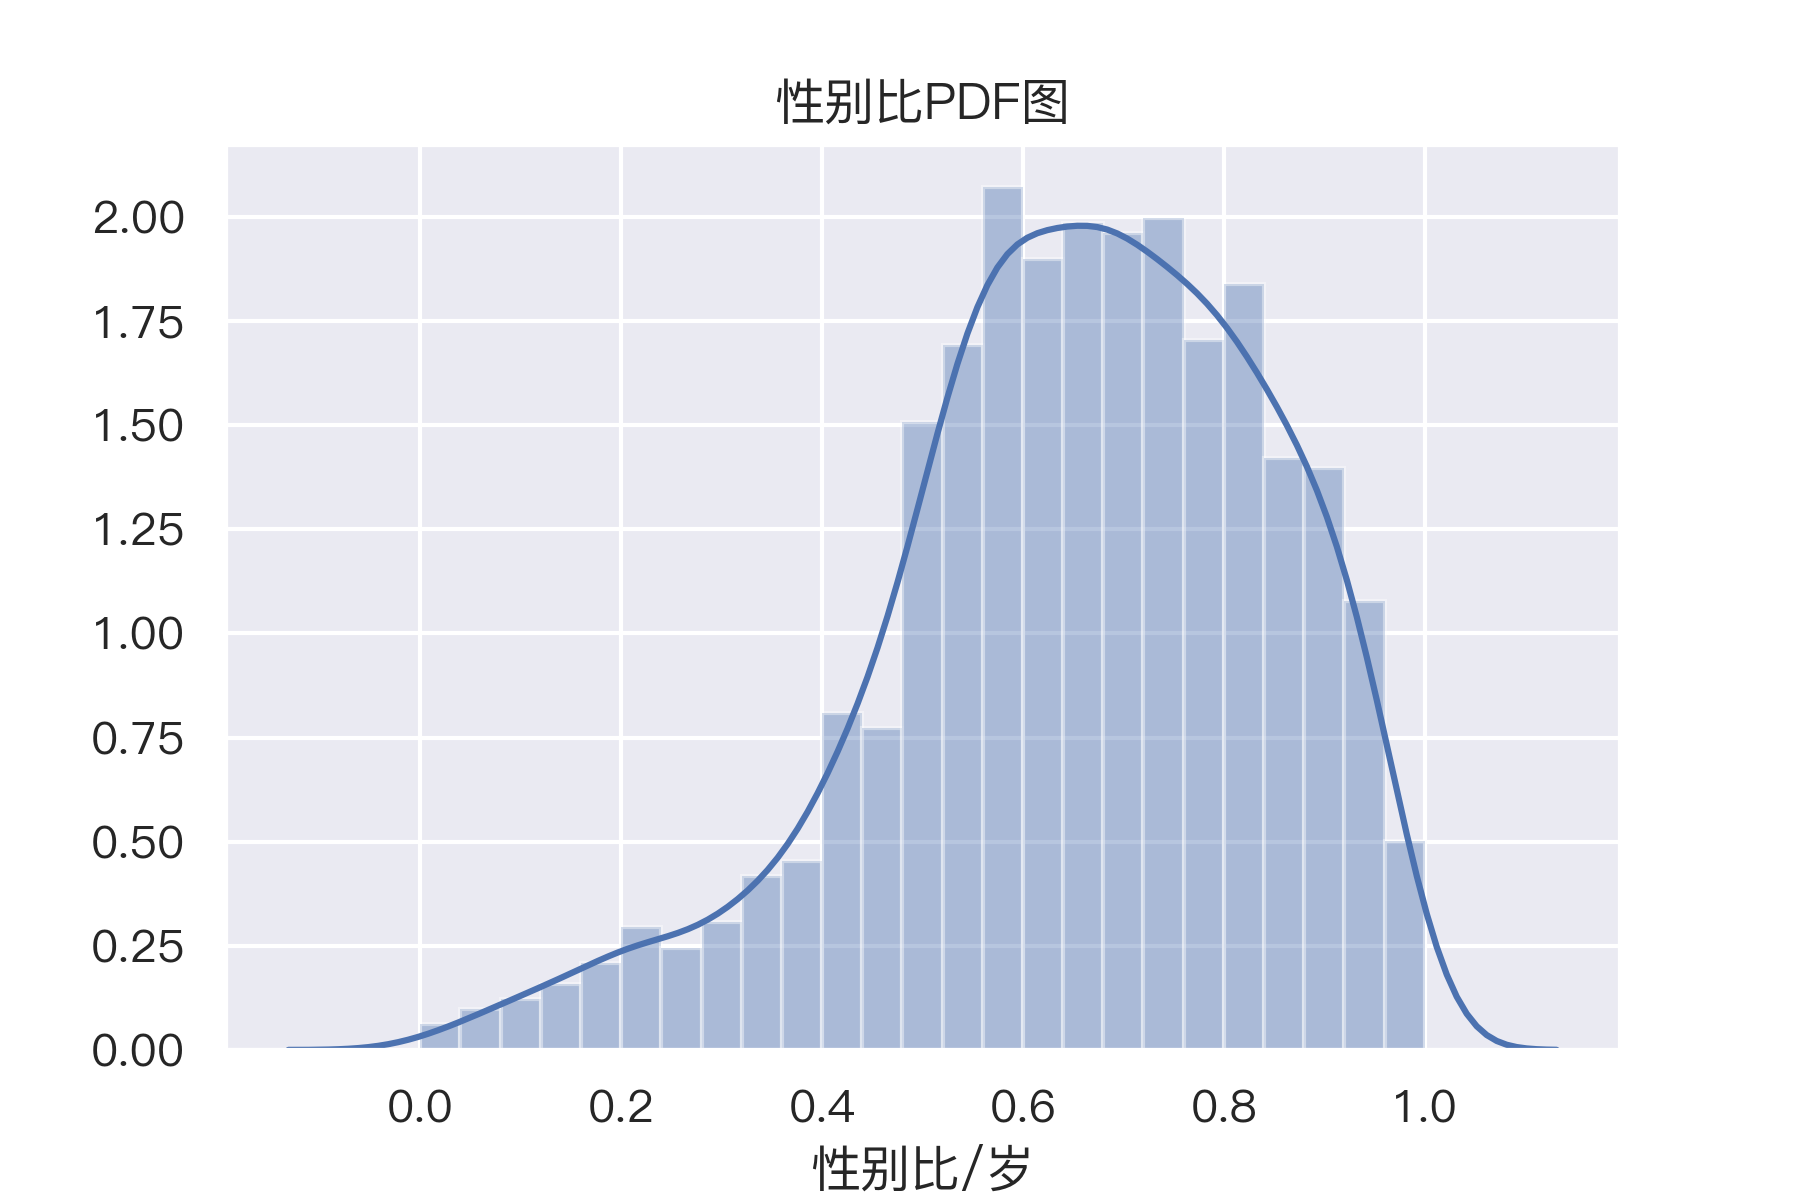
\includegraphics[width=0.95\textwidth]{task5-性别比-pdf}
        \caption{性别比经验概率密度函数}
        \label{fig:gender}
    \end{figure}
    \begin{figure}[htbp]
        \centering
        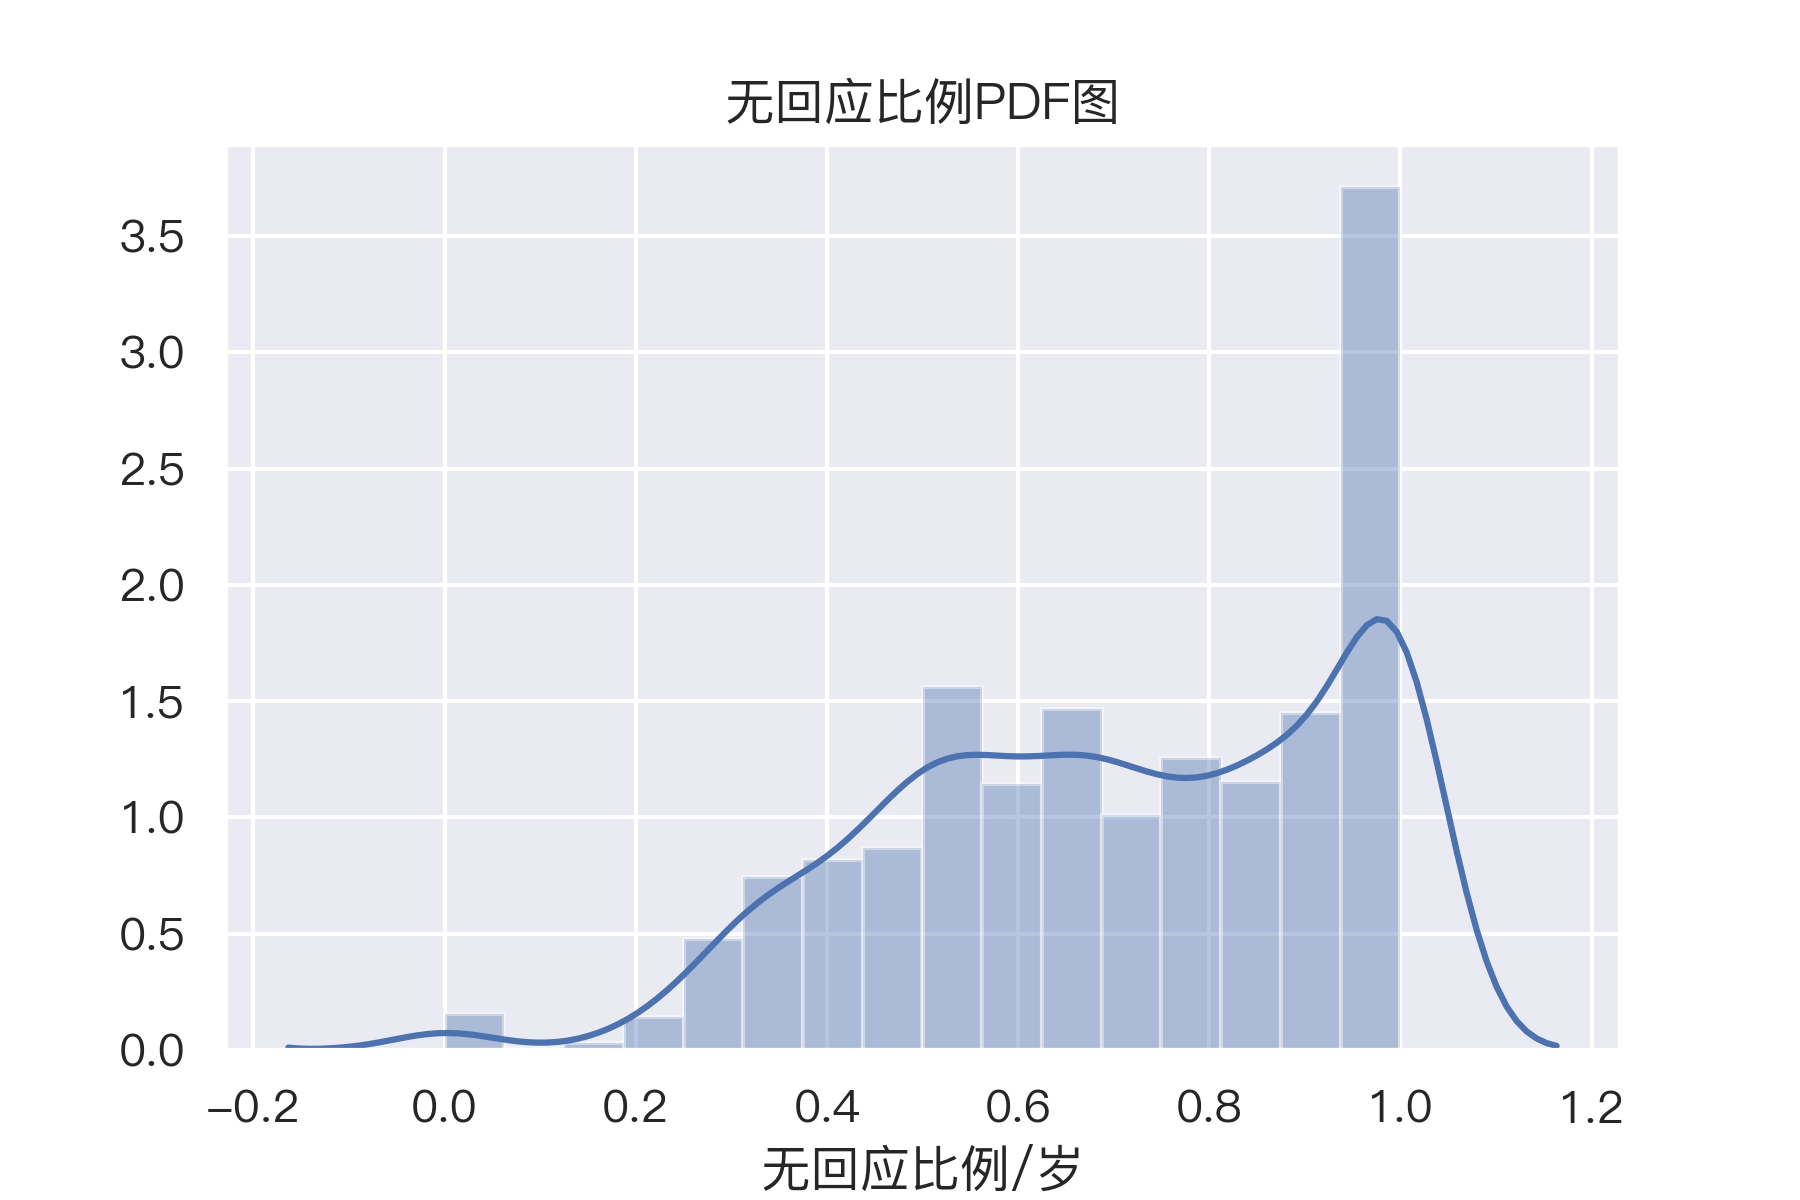
\includegraphics[width=0.95\textwidth]{task5-无回应比例-pdf}
        \caption{无回应比例经验概率密度函数}
        \label{fig:noresponse}
    \end{figure}
    \begin{figure}[htbp]
        \centering
        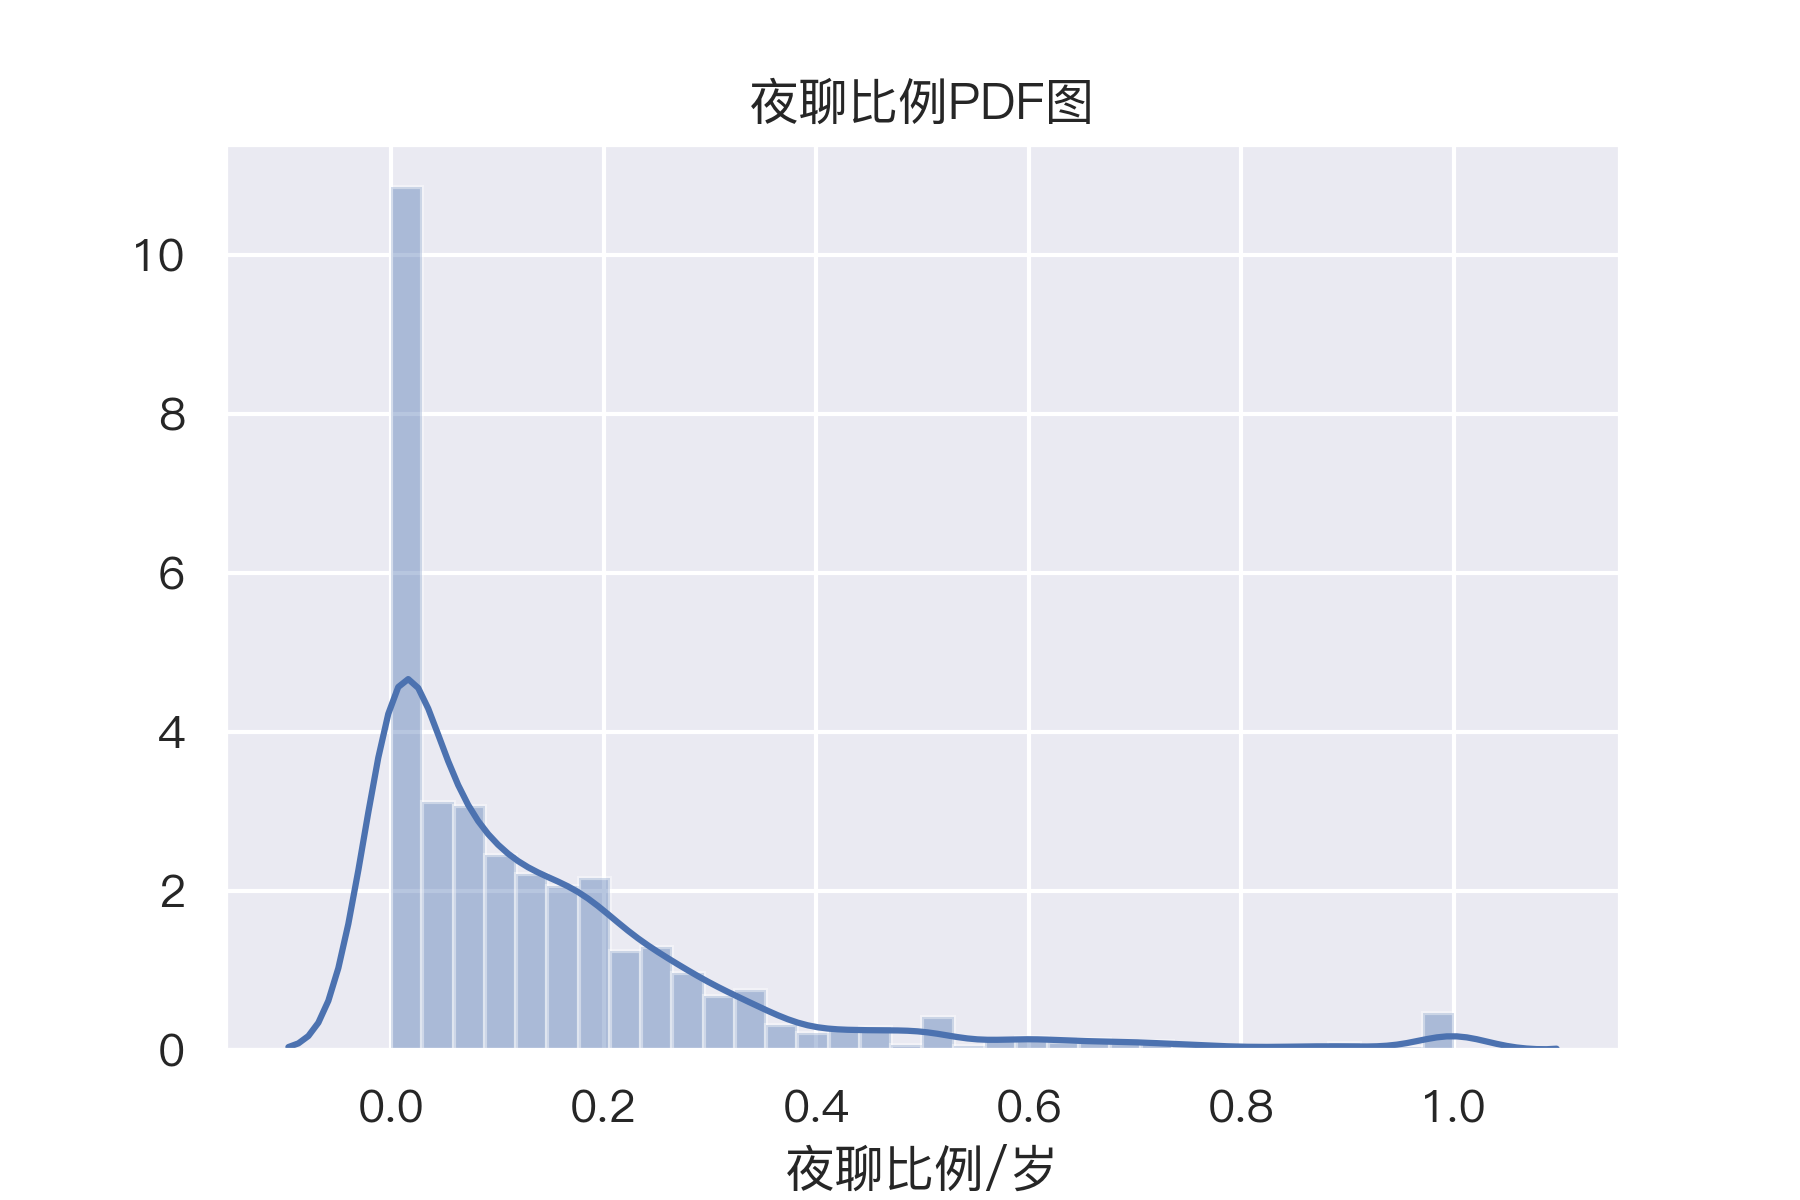
\includegraphics[width=0.95\textwidth]{task5-夜聊比例-pdf}
        \caption{夜聊比例经验概率密度函数}
        \label{fig:nightchat}
    \end{figure}

    针对以上三个特征的正态性进行检验,同样使用偏度-峰度法,得到结果如\cref{task5norm}。结果显示三组均不满足正态性。
    \lstinputlisting[label=task5norm]{task5norm.log}

    \section{任务5} % (fold)
    How to do one-way ANOVA with the non-normal data?
    \subsection{问题1} % (fold)
    \paragraph{问题描述} Find and list the possible solutions set.
    \subsection{问题2}
    \paragraph{问题描述} Do the one-way ANOVA on the 3 columns you choose. Do these feature columns vary significantly? Visualize the results.
    \section{任务6} % (fold)
    \paragraph{问题描述} Redo the ANOVA test in question 3 c) by sampling 10\% data (i.e. around 200 groups). Repeat 10 times and compute the mean and standard deviation of the supporting statistics (F value). Compare at least two sampling strategies. Which sampling method is more stable? How are the results compared to the results without sampling? Why?
    \section{任务7} % (fold)
    \paragraph{问题描述} Choose any two categories, and classify them by logistical regression, or you can try multi-label classification on all categories.
    \label{applastpage}
    \newpage
    \bibliography{report}
    \bibliographystyle{unsrt}
\iffalse
\begin{itemize}[noitemsep,topsep=0pt]
%no white space
\end{itemize}
\begin{enumerate}[label=\Roman{*}.,noitemsep,topsep=0pt]
%use upper case roman
\end{enumerate}
\begin{multicols}{2}
%two columns
\end{multicols}
\fi
\end{document}